%\documentclass{article}
%\usepackage{graphicx,subfigure}
%\usepackage{caption,rotating}
%\begin{document}

\begin{figure}[p]
\centering
 \subfigure[Plate (i) Sheep w479 Wrinkled]{
%   \label{fig:trial1he(i)}
    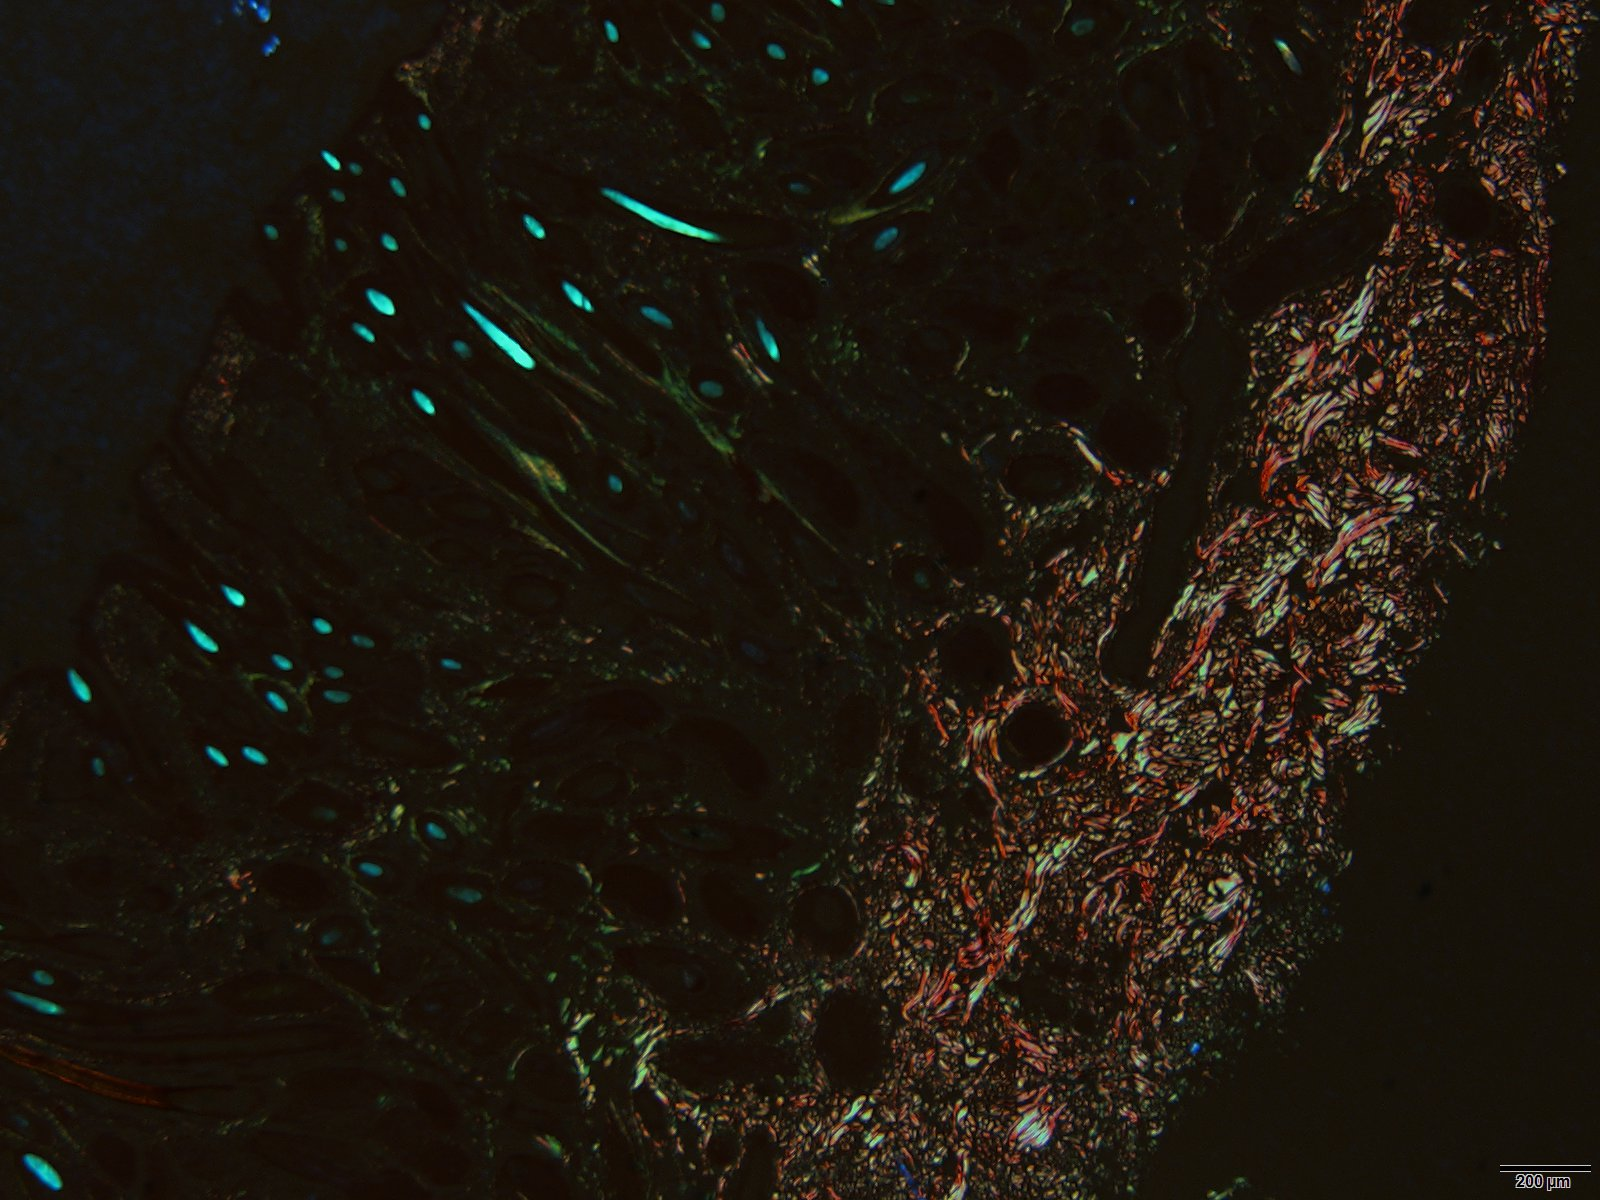
\includegraphics[scale=0.20]{w479-2_rigid_PSR_stain_polarised.jpg}
% 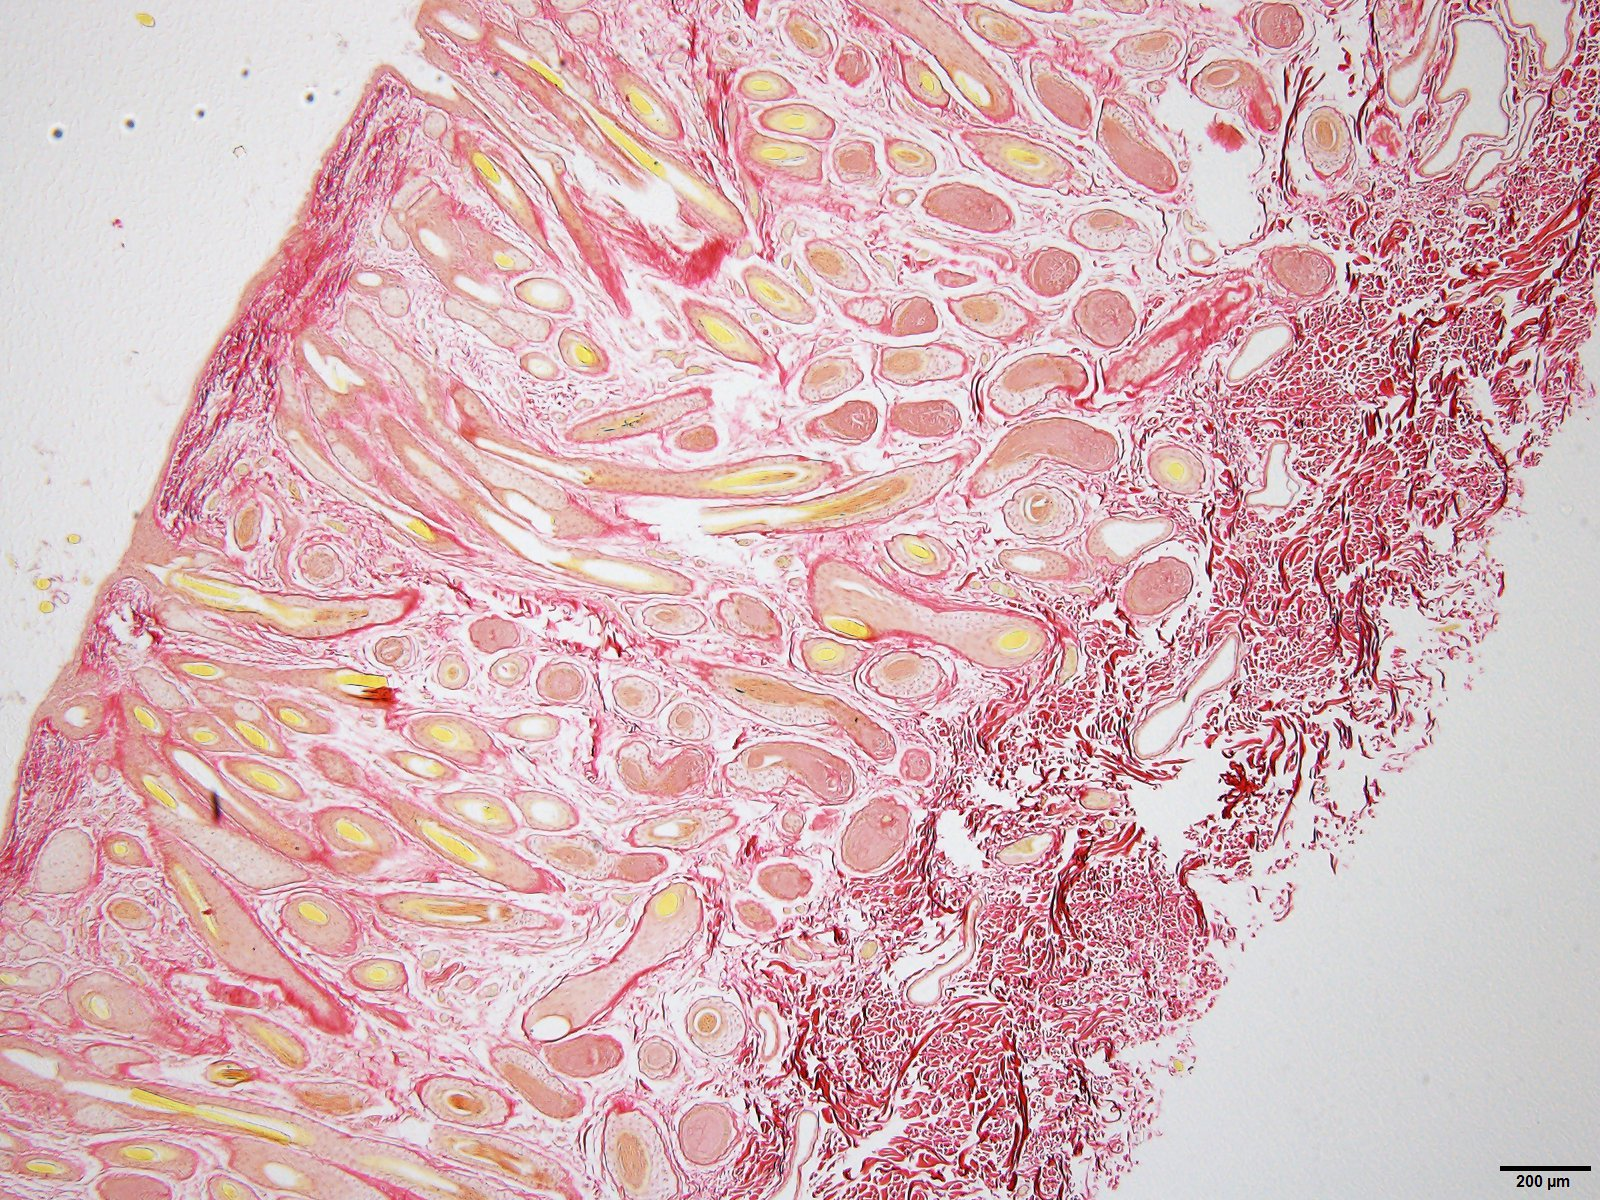
\includegraphics[width=1.0\textwidth]{w479-2-rigid.jpg}
  }
 \subfigure[Plate (ii) Sheep w490 Wrinkle-free]{
%   \label{fig:trial1he(ii)}
    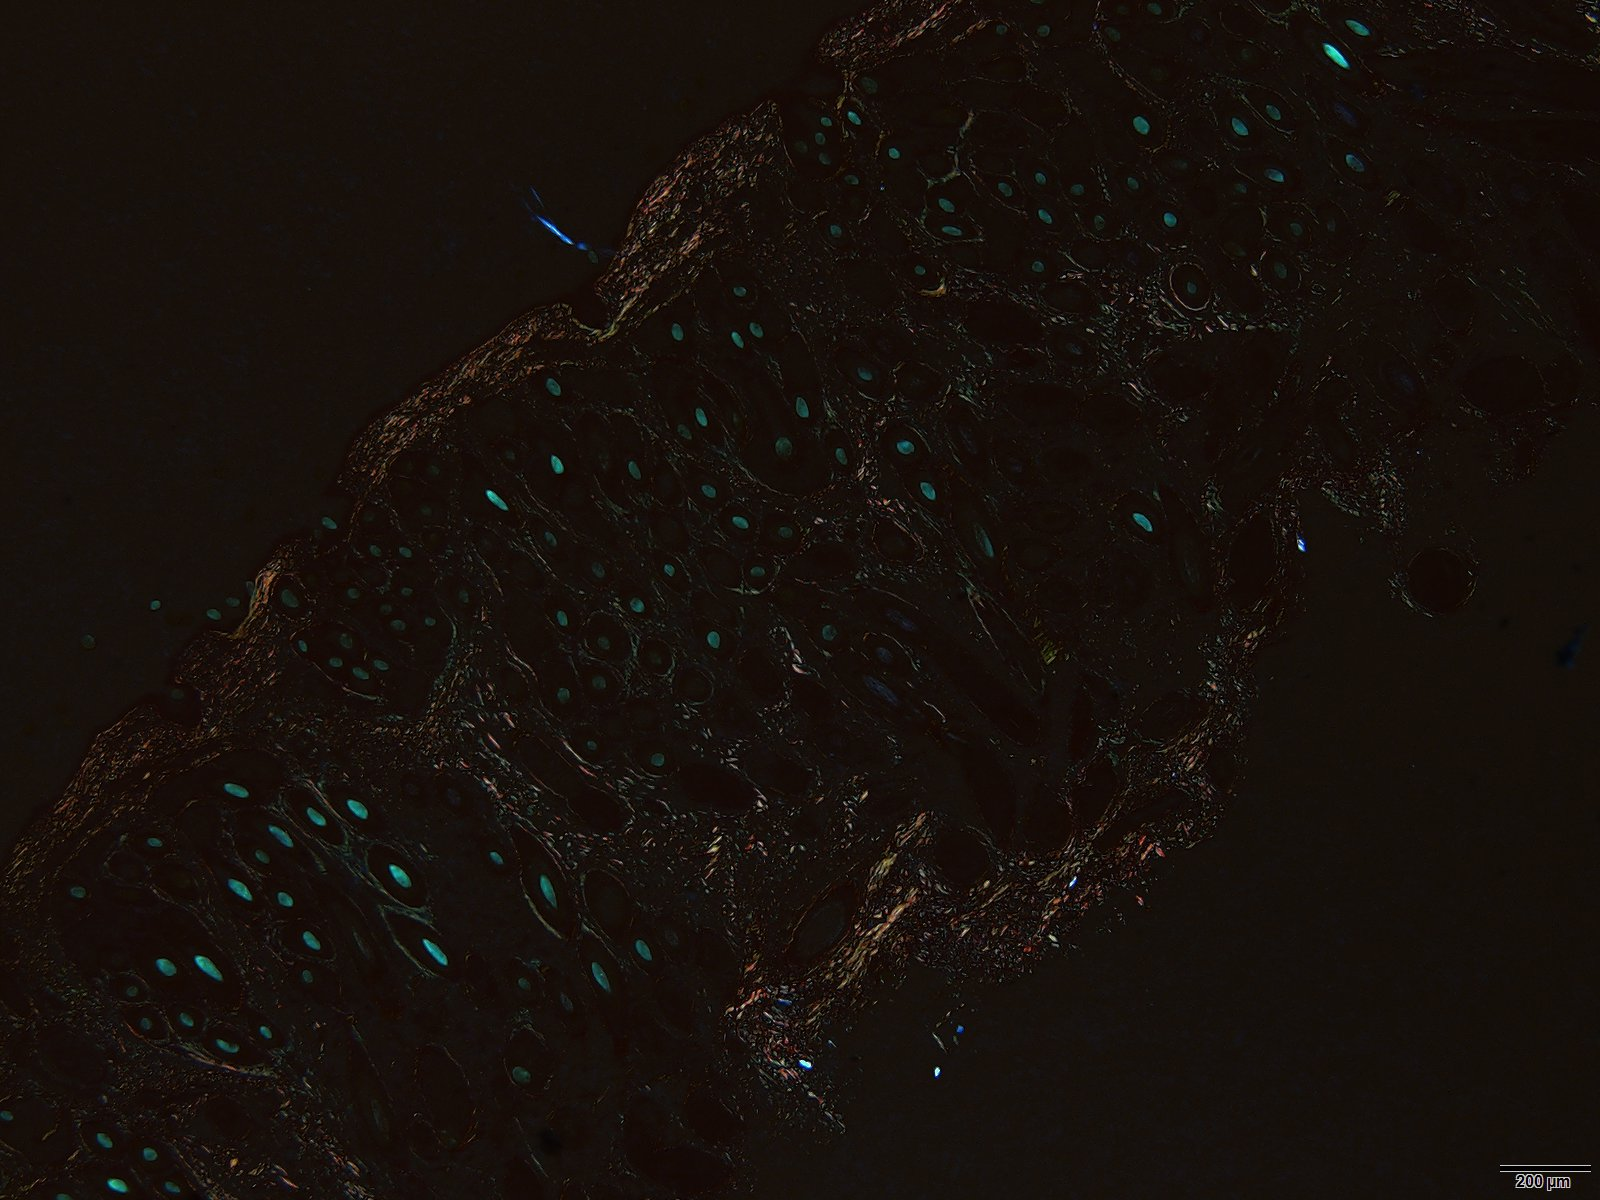
\includegraphics[scale=0.20]{w490-2_supple_PSR_stain_polarised.jpg}
  }
  \caption{Vertical sections from a wrinkled (i) and a wrinkle-free (ii)  sheep from Trial 1 flock 2 stained with PSR and examined with polarised light and a 4x objective. }
\vfill
  \label{fig:polar}
\end{figure}

%\end{document}

